% ------------------------------------------------------------------------------
\section{Resultados} \label{res}

\subsection{Setup do Experimento}

Para a realização do experimento foram utilizadas duas configurações diferentes, ambas consistindo de duas máquinas virtuais idênticas para questões de homologação do protocolo. Para a emulação das máquinas foi utilizado o Qemu. 

A comunicação entre as duas máquinas foi feita através da criação de uma bridge entre as duas e instanciação de uma aplicação contendo o Mestre e outra contendo o Escravo.

As mensagens de sincronização ocorreram a cada 3 segundos, sendo assim cada sincronização pertencente aos gráficos a seguir corresponde à troca de três mensagens de sincronização e quatro {\it timestamps}. Sendo o primeiro {\it  timestamp} equivalente à saída da mensagem de sincronização do nodo mestre, o segundo {\it timestamp} correspondente à chegada da mensagem de sincronização e o terceiro e quarto {\it timastamps}  representam os envios das mensagens para calcular o atraso da rede.


\subsection{Resultados do Experimento}

O primeiro experimento contou com os dois relógios sincronizados desde o início, sendo que a sincronização foi mantida a níveis próximos à 0 segundo durante as 250 sincronizações, como mostra a Figura 5.
		
		\begin{figure}[ht]
				\begin{center}
				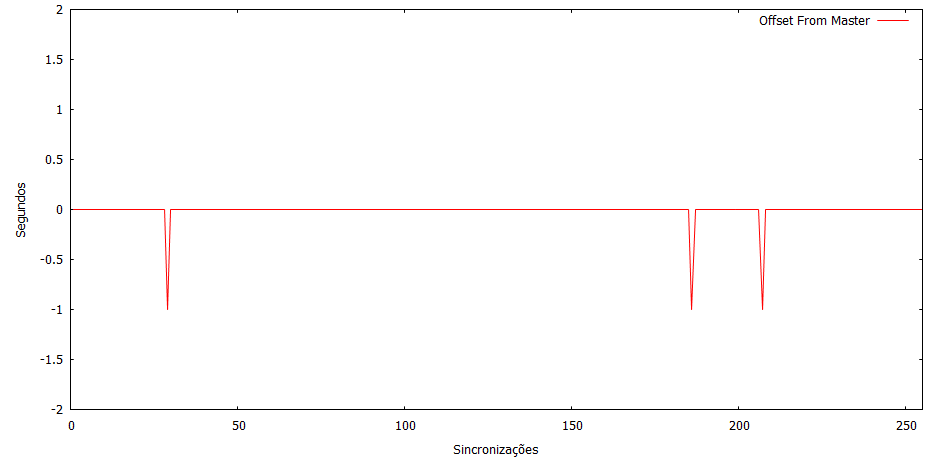
\includegraphics[scale=0.4, width=9cm]{fig/dados7.png}
				\caption{Offset entre dois relógios previamente sincronizados}
				\end{center}
				\end{figure}

Pequenas variações no {\it offset} foram encontradas, um valor equivalente a -1s em três ocasiões. Isto pode ser explicado através de alguns fatores que influenciam a precisão da sincronização como o atraso assimétrico e falhas no relógio.

Após a realização do primeiro experimento, seguimos com o segundo experimento onde contávamos com as duas máquinas virtuais, sendo que o escravo possuía seu relógio atrasado em relação ao mestre. Foi obtido uma variação do {\it offset} entre -1 e 1 segundo, porém logo após a centésima sincronização o {\it offset} começou a se estabilizar, chegando a marca de 0s, mostrando que os mesmos encontram-se sincronizadas na casa de no mínimo Milissegundos, como mostra a figura a seguir. Como observado no primeiro experimento obtemos algumas oscilações após se obter a sincronização, ou seja {\it offset} igual a 0s, que são explicadas da mesma forma.
 
	\begin{figure}[ht]
		\begin{center} 
		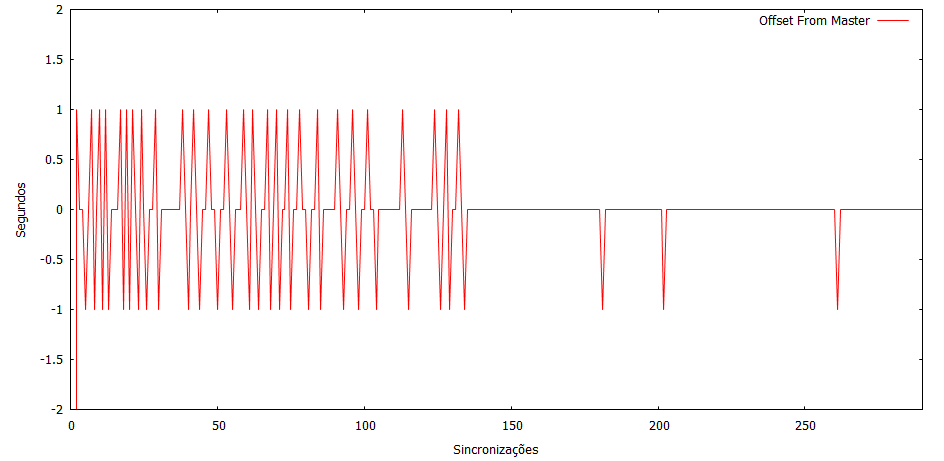
\includegraphics[scale=0.4, width=9cm]{fig/dados8.png}
		\caption{Offset com relógio do escravo atrasado em relação ao relógio do mestre}
		\end{center}
		\end{figure}
		
	O experimento foi repetido, seguindo as mesmas configurações, outras cinco vezes e obteve-se os resultados apresentados nas Figuras 7 e 8, incluindo o desvio padrão dos {\it offsets} calculados e também a média dos {\it offsets} calculados.
	
	\begin{figure}[h!t]
		\begin{center} 
		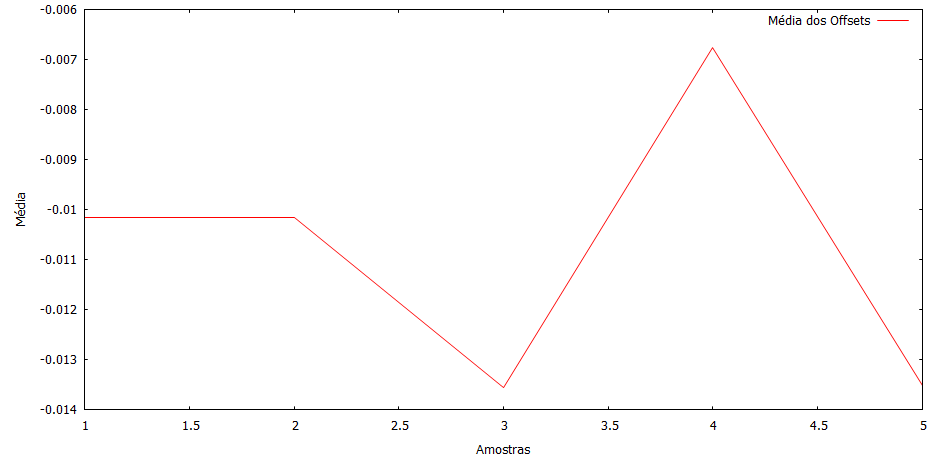
\includegraphics[scale=0.4, width=9cm]{fig/media.png}
		\caption{Média do Offset com relógio do escravo atrasado em relação ao relógio do mestre de 5 experimentos}
		\end{center}
		\end{figure}

	\begin{figure}[h!t]
		\begin{center} 
		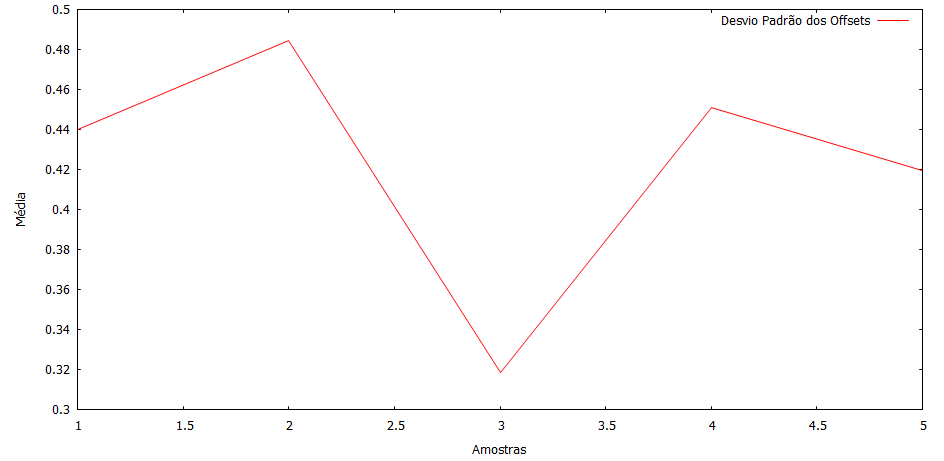
\includegraphics[scale=0.4, width=9cm]{fig/desvpad.png}
		\caption{Desvio Padrão do Offset com relógio do escravo atrasado em relação ao relógio do mestre de 5 experimentos}
		\end{center}
		\end{figure}				
		
	
	Percebemos que a média se mantêm no intervalo [-0.006, -0.014]. Assim podemos dizer que o relógio se manteve na média, quando não sincronizado, à frente do tempo do relógio mestre. Este adiantamento se comprova pelo {\it offset} negativo. Ao analisarmos o desvio padrão observamos que o mesmo está compreendido no intervalo [0.5, 0.3], mostrando assim uma variância entre 0,025 e 0,09 do {\it offset}.

